\section{Problem setting and statistical framework}
\label{sec:procedure}
%%%%
% Background only model determination
Our first step is the determination on the null-hypothesis model, consisting solely 
of Poisson-distributed background emission.
%
To this end, we apply a mask of  $|b|<30^\circ$ around the Galactic plane, and remove the emission of all 
sources in the 4FGL-DR3 catalogue, further masking a $1^\circ$ disk around each source centroid. This cut roughly corresponds to the 90\% containement angle of the PSF and represents a good compromise between removing the bulk of the pointlike emission while avoiding a too large removal of the diffuse emission area. We checked that the results are not particularly sensitive to the exact cut used in the $1^\circ-2^\circ$ range. 
%
%Fit
We then compute the expected photon counts $\lambda_i$ of model $\mathcal{B}$ (depending on $A_\textrm{gal}$  and $ F_{0}$) in the pixel $i$  and, given the actual counts $k_i$, define the Poissonian likelihood  
\begin{equation}
{\cal L}_0=\prod_{i=1}^{N_\textrm{pix}} \frac{\lambda_i^{k_i}e^{-{\lambda_i}}}{k_i!}\, .
\end{equation}
The adopted parameters $A_\textrm{gal}$  and $ F_{0}$ are those maximising the likelihood above. For $N_\textrm{side}=512$, we find $A_\textrm{gal}=0.914$ and $F_0=4.81\cdot 10^{-7}$ cm$^{-2}$ s$^{-1}$ sr$^{-1}$.
%


\medskip
%
Our second step is to quantify the significance of additional point sources on top of the
null-hypothesis model.
%
For this purpose, we define a test statistic ($TS$) function in each pixel, quantifying how well the  observed photon counts agree with the background-only hypothesis:    
\begin{equation}
    TS_i \equiv \frac{(x_i - \lambda_i)^2}{\lambda_i}~,
\label{eq:TS}
\end{equation}
where we indicate with $\lambda_i$ the best-fit background-only model counts in the pixel $i$, computed according to eq.~\eqref{eq:mapB};  $x_i$ can be either the observed photon counts 
(when applied to the actual photon count map of data, leading to the single set $TS^\textrm{data}_i$) or the  photon counts in pixel $i$ generated via synthetic maps. If the maps are generated according to  the hypothesis eq.~\eqref{eq:mapK}, the procedure yields the single set $TS^\textrm{cat}_i$; if the maps are randomly taken from the model of eq.~\eqref{eq:map}, we obtain a number of sets $TS^\textrm{sim}_i$ equal to the number of realisations.
The $TS$ choice of eq.~\eqref{eq:TS} is inspired by Pearson's $\chi^2$ test statistic for Poisson distributed counts,
whose variance $\sigma_i^2=\lambda_i$. 
This choice also loosely mimics the one adopted by the \Fermi-LAT collaboration, albeit no exact correspondence can be expected.  In fact, \Fermi-LAT uses a recursive procedure where, after a first step similar to the above, energy-dependent renormalisations of the background are allowed independently in each ``region of interest''.  We prefer to use a simple and coherent definition valid for all pixels in the sky, also because we do not assume a particular probability distribution for the $TS$ values. Rather, we use it as a ``signal interest label'', and derive a probabilistic interpretation for it from simulations of synthetic maps (see below). 

Obviously, since in our simulations the sources are uniformly distributed across the sky, the spatial distribution of $TS^\textrm{sim}_i$  never coincides with the one obtained from the actual data, $TS^\textrm{data}_i$, nor with the one from the 4FGL-DR3 catalogue, $TS^\textrm{cat}_i$. However \textit{the histogram of the $TS^\textrm{sim}_i$ values should statistically match the actual one $TS^\textrm{data}_i$, if the functional form and inferred parameters of the underlying $\dNdS$ are correct}.  
Since the determination of $\dNdS$ exploits information below the nominal catalogue's threshold, the statistical agreement between the actual map and the synthetic maps should hold at values below this threshold and inform us about new, faint sources. This is the gist of the argument that we exploit to extend \textit{statistically} the \Fermi-LAT catalogue below threshold. This expectation is illustrated in figure~\ref{fig:1}, where we report the descending cumulative $TS$ distribution for real data (black), the 4FGL-DR3 catalogue source model, $\mathcal{K}$ (gray), and for several realisations of the $\dNdS$ source model, $\mathcal{M}$ (blue). While the distributions match rather well at high $TS$, the one associated to the catalogue departs from the data one well before the simulation's ones do. 

\begin{figure}[t]
\centering
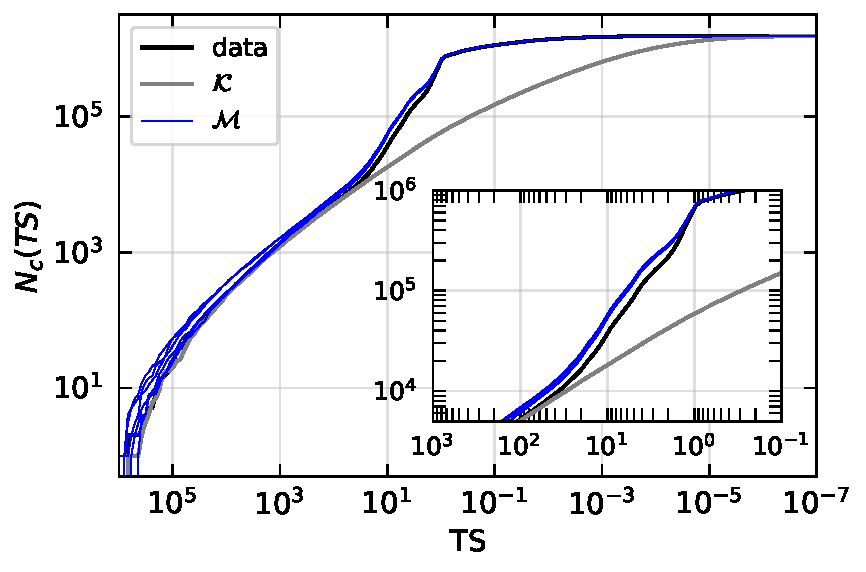
\includegraphics[width=0.6\textwidth]{img/N_c.pdf}
\caption{Descending cumulative $TS$ distribution for the maps corresponding to: real data (black), 4FGL-DR3 catalogue (gray) and a few realisations of the $\dNdS$ source model (blue).
}
\label{fig:1}
\end{figure}

\medskip
%KS test
As a next (and third) step, we attribute a statistical meaning to the $TS$ distributions. 
At large $TS$, we expect the observed map and the simulated ones to  agree well: Visible (but insignificant) discrepancies are expected at the highest values of $TS$, where Poisson fluctuations are important. At low $TS$ we expect the deviations from the two distributions to eventually become statistically significant. This is due to the interplay of the weakness of the sources and the systematic errors in the background template, that are more and more relevant at low fluxes. 

To assess how well the two distributions are in agreement, we apply a two-sample Kolmogorov-Smirnov (KS) test ~\cite{KS_test} to the normalised cumulative distribution functions of real data and simulated sky (or catalogue sky), both cut at a minimum $TS_*$, which we vary on a grid.
Their compatibility depends on the confidence level $1-\alpha$ at which we set the test. This is strictly speaking arbitrary, although conventionally $\alpha$ is set to 0.05 in most applications. We will actually consider three values of $\alpha$: 0.01, 0.05 and 0.1, to assess the dependence of the results on this meta-parameter. In general, increasing $\alpha$ yields more conservative constraints, as the criterion to reject the null hypothesis becomes more restrictive (i.e. the distributions should agree more closely). 

For the single catalogue model in eq.~(\ref{eq:mapK}), we present the results in terms of the $TS_*$ leading to  agreement with real data as a function of $\alpha$. 

In the case of the $\dNdS$ model, since we have multiple realisations, we quantify what is the fraction of simulations which passes the test against the true sky distribution as a function of $TS_*$ (and $\alpha$). This provides a \textit{quality factor} $QF$ that we associate to the considered cut. Lacking a better criterion, a reasonable choice may be to require a majority of realisations to lead to an agreement (i.e. $QF>0.5$), but it is strictly speaking another meta-parameter which depends on the criteria of the user.  We will also show how results depend on $QF$, with $QF$'s closer to 1 associated to more restrictive requirements. Note that we will ``naively'' interpret the $QF$ as probability of the $TS$ being associated to a source, by considering the whole sample of simulations as equally viable (i.e. only the prior information based on the pixel statistics is used). In principle, one could refine this indicator by restricting the sample of simulations to the ones which reproduce the high-$TS$ distribution. We expect the actual probability to be somewhat higher than the one estimated via the $QF$. Also note that nowhere in our procedure we have relied on the 4FGL catalogue as input.~\footnote{Technically, we mask the catalogue position to fit the background model, but this is done only to lead to a better  background model and thus a more meaningful $TS$ scale. In principle, we could fit the background model without masking the catalogue source positions. That would alter our $TS$ scale, but the same bias will affect the simulated sky maps that we use to attribute a statistical meaning to the $TS$.}

The final step is how to identify the ``firing pixels'' in the true sky which are going to constitute the main deliverable of our work. For a fixed KS test significance $\alpha$ and a quality factor QF, we obtain a value $TS_*$ above which a fraction QF of simulations is compatible with the measured sky. Those pixels $i$ in the latter having $TS_i>TS_*$ will simply constitute of candidate pixels.

\medskip
We conclude this section with a general remark. We note that our procedure treats every pixel independently, assigning a $TS$ value to each of them, regardless of the $TS$ values of the neighboring pixels. In this respect, it is  useful to distinguish between a source and a ``firing pixel'': Multiple pixels may be firing (i.e.~having a sufficiently large $TS$) in association to a single source, depending on the choice of $N_\textrm{pix}$, the intensity of the source and the PSF of the instrument (indirectly, thus, also on the spectrum of the source). This instance is more and more likely the smaller the pixel size, i.e.~the larger $N_\textrm{pix}$, is. Conversely, multiple sources may be associated to a single pixel, notably for choices of $N_\textrm{pix}$ which are too low. Clearly, for the exercise proposed here to be useful, we must require that the choice of $N_\textrm{pix}$ leads to a number of pixels in the non-masked sky sufficiently larger than the current number of sources in the catalogue in the same region. At the same time, a pixel size  much smaller than the angular resolution would be meaningless. Keeping this in mind, for the sake of simulations, we fix $N_\textrm{side}=1024$, which corresponds to an angular resolution of approximately $0.06^\circ$, in order to match the angular resolution of the Galactic foreground template. However, since the \Fermi-LAT angular resolution in the (1,10) GeV energy band is at best of the order of $0.15^\circ$ \footnote{\href{https://fermi.gsfc.nasa.gov/science/instruments/table1-1.html}{https://fermi.gsfc.nasa.gov/science/instruments/table1-1.html}}, for the sake of our pixel analysis, we will downgrade our simulations to $N_\textrm{side}=512$, which corresponds to an angular resolution of approximately $0.12^\circ$. The choice of this value for $N_\textrm{side}$ ensures that there are considerably more pixels than the number of resolved sources (approximately 500 times the number of resolved sources in the region $|b|>30^\circ$) and that the pixel size  of our analysis roughly matches the best resolution of the LAT at the energies of interest.
The $TS$ analysis is therefore performed with synthetic and real data maps pixelized with $N_\textrm{side}=512$.


%%%%

